\section{Introduction}

	Astrophysical and cosmological observations present evidence that 27\% of the mass-energy of the Universe is made out of Dark Matter (DM), a non-luminous, non-baryonic and non-relativistic particle, though the nature of this particle is yet unknown~\cite{Harvey1462}. While several types of new DM candidate raise from many theories, the most prominent one is the Weakly Interacting Massive Particles(WIMPs)~\cite{Bertone:2010zza}. Many  direct detection experiments attempt to measure the rare scattering of WIMPs from target nucleus. Although some experiment see an excess for WIMPs in the mass range of 6-30 GeV/$C^2$~\cite{DAMA,COGENT,CDMSlite,CREST}, these results are in tension with other experiments~\cite{xe100_run_combination,PANDAX,LUXnew}.
	
	 Typically the standard calculation for WIMP nucleon scattering simplifies the type of interaction to Spin Independent (SI) and Spin Dependent (SD) interactions~\cite{LEWIN}, however these are not the only possible types of interactions. In recent years an Effective Field Theory (EFT) approach that takes into account all leading-order and next-to-leading order operators that emerge from the effective Lagrangian and describes the WIMP-nucleus Interaction, has been developed ~\cite{Fitzpatrick:2012ib,Anand:MathTools,Fitzpatrick:MathTools}. In this framework new operators which come from different type of nuclear responses are introduced along with the standard SI and SD ones. The parametrization of the fourteen operators $O_i$ is listed in Eq.~\ref{eq:OpDef} and follows the convention from~\cite{Anand:MathTools}. The operators dependence explicitly on 4 quantities $\vec{v}^{\perp}$, the relative velocity between the WIMP and the nucleon, $\vec{q}$, the momentum transfer, and the WIMP and nucleon spin $\vec{S}_\chi$ , $\vec{S}_N$. Notice that $O_2$ is not treaded as it cannot be obtained from a relativistic operator at leading order.
	 
	    Unlike The standard type of interactions which has no dependent on the momentom transfer and therefore most of the interaction rate will be in low energies, some of the new operators do depend on $\vec{q}$ the interaction rate peaks at higher energies then looked in direct detection experiments ($< 40$ keV), and hence could not be treated before see Fig. ~\ref{fig:dRdE}.
	    
	    Another assumption that can be relaxed is that WIMP should scatter elastically, however there are models in which the incoming and outcoming WIMPs have different masses ~\cite{InelasticIntro}. In this scenario low recoil energy is very suppressed, Hence experiments which apply a high energy bound loss sensitivity to these types of interactions. Lately an adaptation to the elastic EFT operators was developed~\cite{InelasticMath}. The operators presented in ~\ref{eq:OpDef} are modified such $\vec{v}^\perp_{inelastic} = \vec{v}^\perp_{elastic} +\frac{\delta}{\vert{\vec{q}}\vert^2}\vec{q}$.      
	    
	    In this paper we report on an analysis enlarging the energy range up to 240keV for the first time in \Xehund\ experiment. and present exclusion limits on all operators for both the elastic case and the inelastic one in a model independent way.     

\begin{equation} \label{eq:OpDef}
\begin{split}
O_1 &= 1_{\chi} 1_N  \\
O_2 &= (v^{\perp})^2 \\
O_3 &= i\vec{S}_N\cdot (\frac{\vec{q}}{m_N}\times\vec{v}^\perp) \\
O_4 &= \vec{S}_{\chi}\cdot \vec{S}_N \\
O_5 &= i\vec{S}_{\chi}\cdot (\frac{\vec{q}}{m_N}\times\vec{v}^\perp) \\O_6 &= (\vec{S}_{\chi} \cdot \frac{\vec{q}}{m_N})(\vec{S}_N \cdot \frac{\vec{q}}{m_N}) \\
O_7 &= \vec{S}_N \cdot \vec{v}^\perp \\
O_8 &= \vec{S}_{\chi} \cdot \vec{v}^\perp \\
O_9 &= i\vec{S}_{\chi} \cdot(\vec{S}_N \times \frac{\vec{q}}{m_N}) \\
O_{10} &= i\vec{S}_N \cdot (\frac{\vec{q}}{m_N}) \\
O_{11} &= i\vec{S}_{\chi} \cdot (\frac{\vec{q}}{m_N}) \\
O_{12} &= \vec{S}_\chi \cdot (\vec{S}_N \times \vec{v}^\perp) \\
O_{13} &= i(\vec{S}\chi \cdot \vec{v}^\perp)(\vec{S}_N \times \frac{\vec{q}}{m_N})\\
O_{14} &= i(\vec{S}_\chi \times \frac{\vec{q}}{m_N})(\vec{S}_N \cdot \vec{v}^\perp) \\
O_{15} &= -(\vec{S}_\chi \times \frac{\vec{q}}{m_N})[(\vec{S}_N \times \vec{v}^\perp)\cdot \frac{\vec{q}}{m_N}]
\end{split}
\end{equation}
	        	       
%  \begin{itemize}
%  \item Motivation: dark matter, theoretical possibility of high energy recoil events. Mention some specific models, maybe inelastic scattering also.
%  \item Theoretical background on EFT operators, inc. motivation (e.g. possibility to reconcile limits vs possible signals in other experiments, model-independent approach to constraining exotic models)
%  \item (if we do it) Theoretical background on inelastic scattering kinematics.
%  \item Motivating example plots of recoil spectra/signal models (e.g. Fig. \ref{fig:dRdE}). Also discuss the lower electronic recoil background at these higher recoil energies, which improves the analysis sensitivity beyond what would be expected from the raw increase in predicted event rate (At least I presume so, need to estimate this perhaps. I think we can say something like this; the standard analysis signal region has a signal acceptance of maybe 50\% since it cuts the nuclear recoil band about in half, whereas for us it is almost 90\% since there is good separation between ER and NR bands. So for say O3 (either mass) we expect about twice as many events due to the extended signal region, with twice the acceptance in the new high PE region. So overall I guess it is roughly a factor of 3 improvement in total signal rate, and similar for the sensitivity. In fact from the proper sensitivity estimates the improvement is a little better than that, but this gives a rough idea where the improvement comes from.).
% \end{itemize}


\begin{figure}[h!]
\begin{minipage}{1.\linewidth}
\centerline{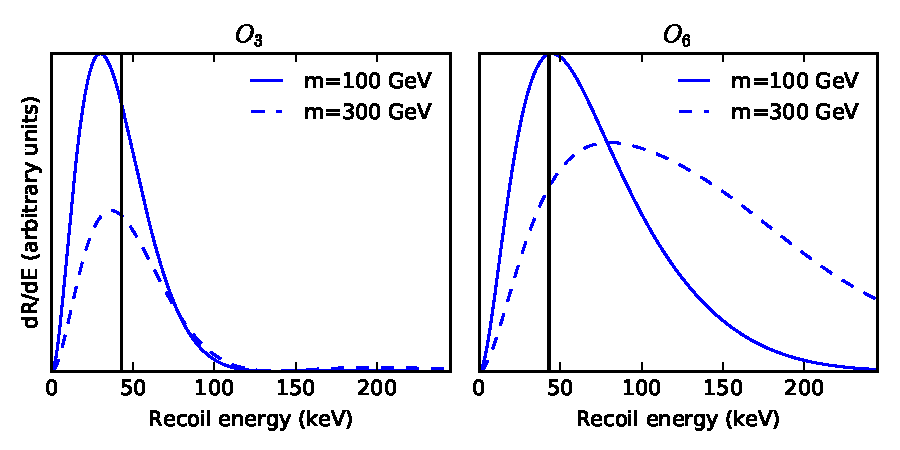
\includegraphics[width=1.\linewidth]{Figures/dRdE_examples.pdf}}
\end{minipage}
\caption{Example EFT recoil spectra for elastic scattering of spin-$1/2$ WIMPs on Xenon nuclei (weighted according to the isotope abundances in the XENON100 experiment). Left(right) shows the predicted spectra for EFT operate $O_3$($O_6$). The normalization is controlled by the coupling coefficient of each EFT operator and the experimental exposure (left arbitrary in this figure). The solid vertical line at 43 keV shows the approximate division between the two signal regions used in this analysis (30 PE in cS1). As shown, certain EFT operators, for certain WIMP masses, predict a significant fraction of recoil events above the upper energy cut used in the standard spin-independent analysis, motivating an extension of this cut. The highest recoil energy shown in the plots, 240 keV, roughly corresponds to the extended $cS1$ cut of 180 PE used in this analysis.}
\label{fig:dRdE}
\end{figure}

\FloatBarrier
\section{The \Xehund\  Detector}
The \Xehund\ detector is a cylindrical (30cm height X 30cm diameter) dual phase Xenon Time Projection Chamber (TPC) that holds 62 kg of Liquid \Xe\ (LXe) targets ~\cite{xe100_instr2012}. It operates at the Laboratori Nazionali del Gran Sasso (LNGS) in Italy. The detector consists a total of 242 1”-square Hamamatsu R8520-AL photomultiplier tubes (PMTs) employed in two arrays, at the top part (in the gas phase) and in the bottom immersed in LXe. a Particle interacting with the LXe deposits energy that creates both excited and ionized states. De-excitation creates a prompt scintillation signal ($S1$). ,  Ionized electrons are drifted in an electric field of $530$V/cm towards the liquid-gas interface, where they are extracted via a larger electric field of $\sim12$kV/cm. These electrons generates a proportional scintillation, which is called $S2$. The spatial distribution of the $S2$ signal on the top PMT array, determines the X-Y position, while the time difference between the two signals gives the z-coordinate, and thus a 3D position reconstructions is achieved.

The ratio of S2/S1 is different weather the interaction is nuclear recoil (NR) or electronic recoil (ER) and thus this ratio is used as a discriminator between ER background coming from $\gamma$, $\beta$ and NR signal coming from a WIMP. 

In previous \Xehund\ analyses the determination of the recoil energy was based on the size of S1 and the scintillation efficiency for the nuclear recoils, \Leff ~\cite{xe100_run10_si}. However in the last analysis ~\cite{xe100_run_combination} a new method was adopted taking into advantage also the S2 signal.
      

